\subsection{Порівняння з LLM-системами перекладу}
\label{subsec:llm_comparison}

Після аналізу результатів основного pipeline (Whisper + OPUS-MT)
та каскадного ефекту постає питання: чи можна значно покращити якість
MT-ланки, замінивши спеціалізовану NMT-модель на сучасну велику мовну модель?
Для відповіді на це питання проведено додатковий порівняльний експеримент
із трьома провідними LLM-системами.

\subsubsection{Опис LLM-систем}

\paragraph{GPT-4o (OpenAI).}
GPT-4o~\cite{gpt4} --- велика мовна модель загального призначення з
авторегресивною Transformer-архітектурою (decoder-only) та контекстним
вікном 128K токенів. За різними джерелами~\cite{hendy_llm_mt}, LLM-based
переклад для пари uk$\to$en досягає BLEU 35--45, а за результатами
людського оцінювання часто перевищує спеціалізовані NMT-системи завдяки
кращому розумінню контексту та здатності до disambiguation~\cite{llm_mt}.

\paragraph{Claude Sonnet 4 (Anthropic).}
Модель використовує авторегресивну Transformer-архітектуру (decoder-only)
з контекстним вікном 200K токенів.

\paragraph{Gemini 2.0 Flash (Google).}
Gemini 2.0 Flash --- швидка мультимодальна модель від Google з контекстним
вікном 1M токенів. Модель оптимізована для швидкого інференсу при збереженні
високої якості генерації тексту.

Зведену характеристику систем наведено у таблиці~\ref{tab:mt_comparison}.

\begin{table}[h]
\centering
\caption{Порівняльна характеристика MT-систем}
\label{tab:mt_comparison}
\small
\begin{tabular}{|l|c|c|c|c|}
\hline
Характеристика & OPUS-MT & GPT-4o & Claude S.~4 & Gemini 2.0\\
\hline
Тип & Спеціаліз. NMT & LLM & LLM & LLM\\
Архітектура & Enc-Dec & Dec-only & Dec-only & Dec-only\\
Ліцензія & MIT & API & API & API\\
Локальна робота & Так & Ні & Ні & Ні\\
Контекст (токени) & 512 & 128K & 200K & 1M\\
\hline
\end{tabular}
\end{table}

\subsubsection{Умови експерименту}

Для LLM-систем використано параметр \texttt{temperature=0} для забезпечення
максимальної детермінованості. Усі LLM отримували однаковий системний промпт
із інструкціями щодо збереження власних назв, географічних назв та військової
термінології. Вхідними даними слугували ті ж самі ASR-транскрипції
(вихід Whisper), що використовувались для OPUS-MT. Це гарантує
коректність порівняння.

\subsubsection{Результати автоматичних метрик}

Зведені результати оцінювання якості перекладу наведено в таблиці~\ref{tab:llm_comparison}.

\begin{table}[H]
\centering
\caption{Порівняння якості перекладу: OPUS-MT vs LLM}
\label{tab:llm_comparison}
\begin{tabular}{|l|c|c|c|}
\hline
\textbf{Модель} & \textbf{BLEU} & \textbf{BERTScore-F1} & \textbf{METEOR} \\
\hline
OPUS-MT & 23,12 & 0,397 & 0,452 \\
GPT-4o & \textbf{57,00} & 0,725 & 0,746 \\
Claude Sonnet 4 & 55,46 & 0,710 & 0,730 \\
Gemini 2.0 Flash & 56,92 & \textbf{0,739} & \textbf{0,747} \\
\hline
\end{tabular}
\end{table}

Результати показують значну перевагу LLM-систем над спеціалізованою
MT-моделлю OPUS-MT за всіма метриками:
\begin{itemize}[nosep]
    \item \textbf{BLEU}: покращення на 140--147\% (з 23,12 до 55--57);
    \item \textbf{BERTScore-F1}: покращення на 79--86\% (з 0,397 до 0,71--0,74);
    \item \textbf{METEOR}: покращення на 62--65\% (з 0,452 до 0,73--0,75).
\end{itemize}

Статистичну значущість різниці підтверджено кількома непараметричними
тестами. Критерій Манна-Уітні~\cite{mann_whitney} показав $U = 0$ та
$p < 0,001$ для всіх порівнянь OPUS-MT з кожною LLM за кожною метрикою,
що означає повну відсутність перетину розподілів (розмір ефекту
$r = 1,0$). Тест Вілкоксона для парних порівнянь ($W = 0$, $p < 0,001$)
підтвердив ці результати. Тест Крускала-Волліса для порівняння трьох LLM
між собою не виявив статистично значущих відмінностей
($H = 1,08$, $p = 0,58$ для BLEU; $H = 2,37$, $p = 0,31$ для BERTScore;
$H = 1,02$, $p = 0,60$ для METEOR), що підтверджує приблизну рівноцінність
LLM-систем для даної задачі.

\subsubsection{Аналіз покращень}

Візуалізацію відносного покращення LLM над OPUS-MT наведено на рис.~\ref{fig:llm_improvement}.

\begin{figure}[H]
\centering
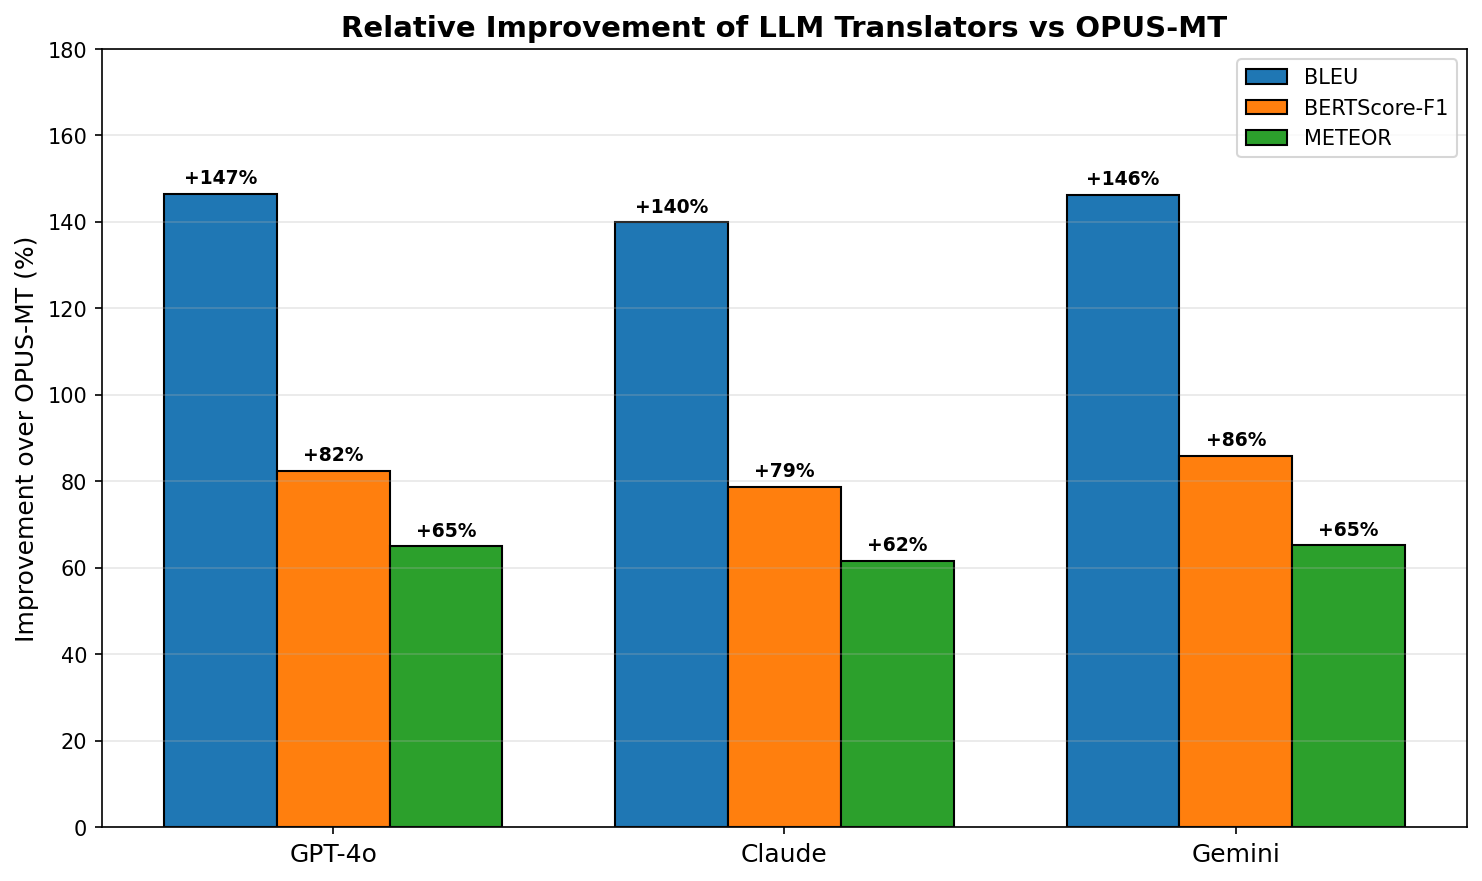
\includegraphics[width=0.9\textwidth]{figures/llm_improvement_percent.png}
\caption{Відносне покращення якості перекладу LLM порівняно з OPUS-MT (\%)}
\label{fig:llm_improvement}
\end{figure}

Серед трьох LLM спостерігається незначна варіація результатів:
\begin{itemize}[nosep]
    \item \textbf{GPT-4o} показує найвищий BLEU (57,00), що вказує
    на кращу лексичну відповідність референсному перекладу;
    \item \textbf{Gemini 2.0 Flash} має найвищі BERTScore-F1 (0,739)
    та METEOR (0,747), що відповідає кращій семантичній подібності;
    \item \textbf{Claude Sonnet 4} показує дещо нижчі результати, але залишається
    кращим за OPUS-MT.
\end{itemize}

Різниця між LLM не є статистично значущою ($p > 0,05$), що дозволяє
вважати їх приблизно рівноцінними для даної задачі.

\subsubsection{Посегментний аналіз}

Порівняння BLEU за окремими сегментами наведено на рис.~\ref{fig:llm_by_segment}.

\begin{figure}[H]
\centering
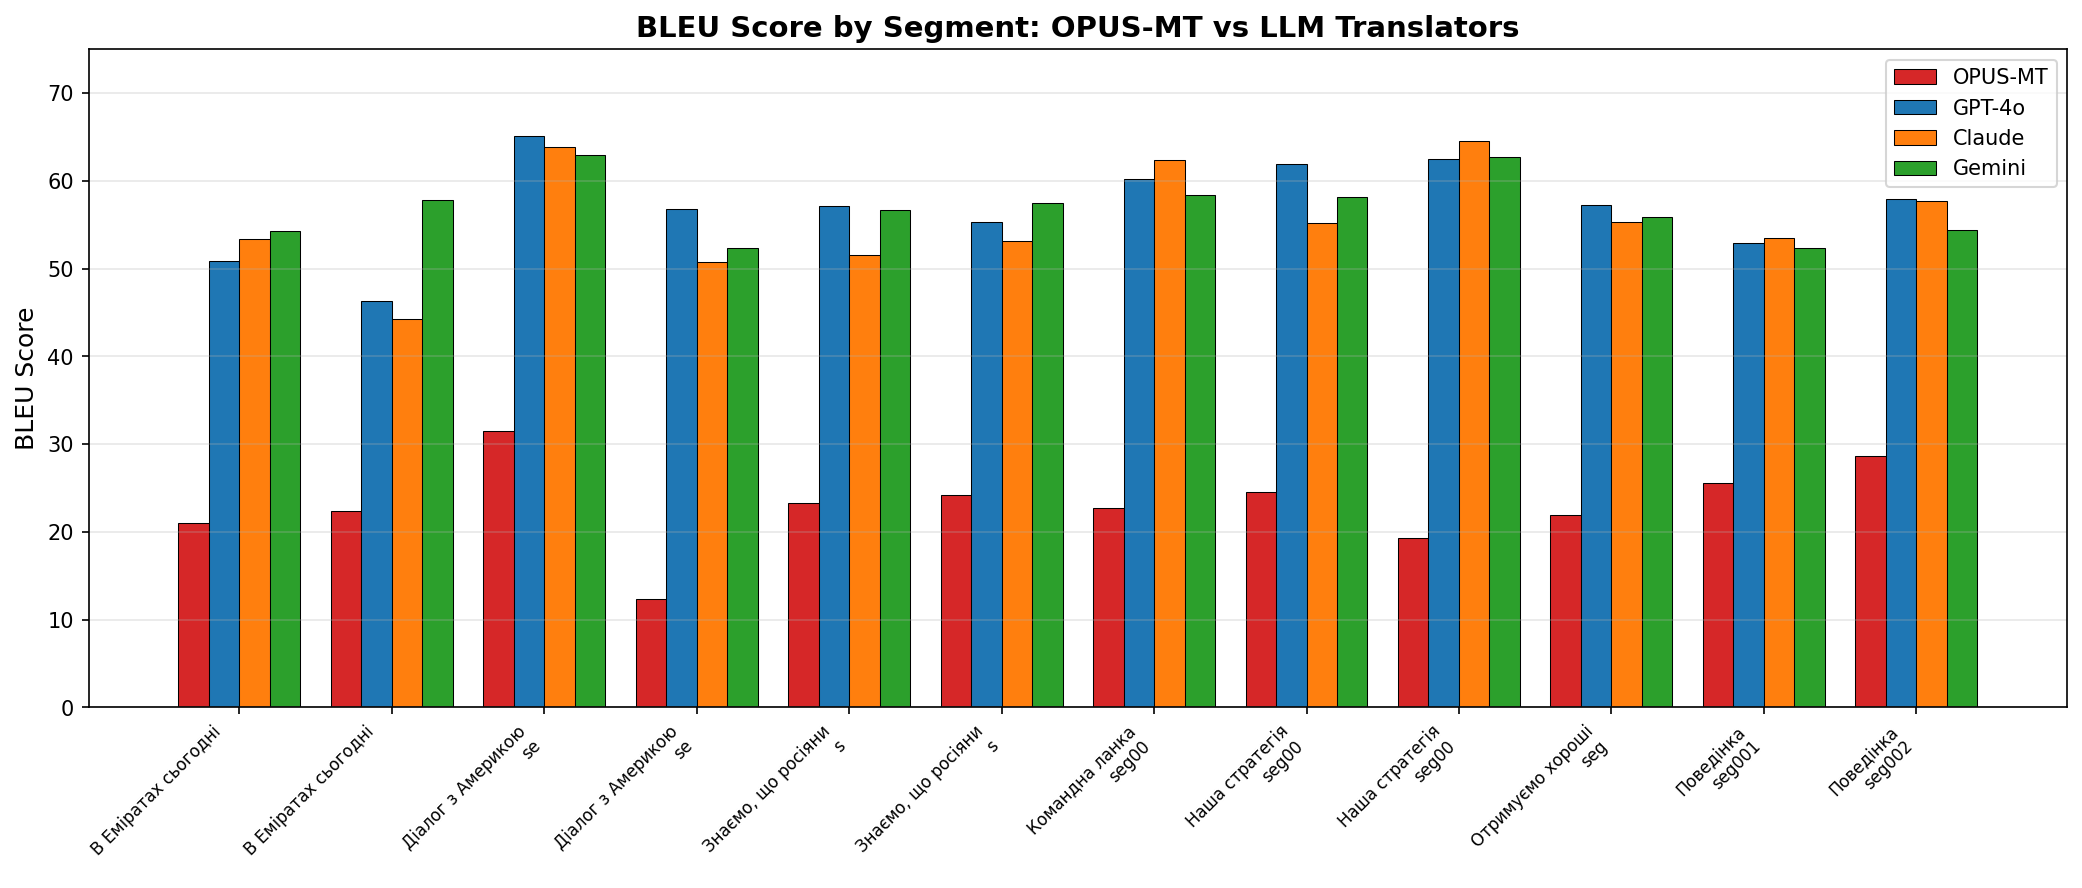
\includegraphics[width=\textwidth]{figures/llm_bleu_by_segment.png}
\caption{BLEU за сегментами: OPUS-MT vs LLM-системи}
\label{fig:llm_by_segment}
\end{figure}

LLM показують стабільно вищі результати на всіх сегментах корпусу.
Особливо помітна перевага на сегментах із високою щільністю власних назв
та термінології (<<Командна ланка>>, <<Наша стратегія>>), де OPUS-MT
показував найнижчі результати.

\subsubsection{Якісний аналіз перекладу власних назв}

Ключовою перевагою LLM є коректна обробка власних назв. Приклади порівняння
наведено в таблиці~\ref{tab:llm_names_comparison}.

\begin{table}[h]
\centering
\caption{Порівняння перекладу власних назв: OPUS-MT vs LLM}
\label{tab:llm_names_comparison}
\small
\begin{tabular}{|p{3cm}|p{3.5cm}|p{3.5cm}|p{3.5cm}|}
\hline
\textbf{Оригінал (ASR)} & \textbf{OPUS-MT} & \textbf{GPT-4o} & \textbf{Референс} \\
\hline
Рустему Міров & Rustema Mirov & Rustem Umerov & Rustem Umerov \\
\hline
Кривирі & Crete & Kryvyi Rih & Kryvyi Rih \\
\hline
генерал Гнатов & General Gnatov & General Hnatov & General Hnatov \\
\hline
ГУР & MBI & HUR (Defense Intelligence) & HUR \\
\hline
\end{tabular}
\end{table}

LLM здатні:
\begin{enumerate}[nosep]
    \item Розпізнавати та коригувати помилки ASR у власних назвах;
    \item Застосовувати стандартну транслітерацію українських топонімів;
    \item Правильно розшифровувати українські абревіатури.
\end{enumerate}

Це пояснюється знаннями, отриманими LLM під час навчання на великих
корпусах, що включають українські та міжнародні новини.

\subsubsection{Обговорення результатів}

\textit{Методологічне зауваження щодо можливого bias:} референсні
переклади для даного дослідження були підготовлені в тому ж числі за допомогою LLM, з подальшою ручною верифікацією. Це може створювати
стилістичний bias на користь LLM-систем, оскільки BLEU вимірює збіг
$n$-грам, а LLM-переклади можуть стилістично наближатися до
LLM-генерованих референсів. Зокрема, метрика BLEU є найбільш чутливою
до цього ефекту через пряме порівняння лексичних одиниць, тоді як
BERTScore та METEOR, що враховують семантичну подібність та синоніми
відповідно, є менш залежними від стилістичного збігу. Слід зазначити,
що перевага LLM підтверджується і за цими метриками (+79--86\% для
BERTScore, +62--65\% для METEOR), а якісний аналіз
(таблиця~\ref{tab:llm_names_comparison}) підтверджує реальну перевагу
LLM у фактичній коректності перекладу власних назв та термінології,
яка не може бути пояснена лише стилістичним bias. Тим не менш,
абсолютні значення метрик слід інтерпретувати з урахуванням цього
обмеження; для остаточного підтвердження масштабу переваги необхідне
порівняння з незалежними професійними референсними перекладами.

Значна перевага LLM над OPUS-MT~\cite{opus_mt} пояснюється кількома факторами:

\begin{enumerate}
    \item \textbf{Масштаб навчальних даних}: LLM навчались на корпусах,
    що на кілька порядків перевищують паралельні корпуси для OPUS-MT.

    \item \textbf{Знання про світ}: LLM мають інформацію про
    українських політиків, географію та військову термінологію, отриману
    під час навчання.

    \item \textbf{Інструкційне налаштування}: можливість надати LLM
    детальні інструкції щодо стилю та специфіки перекладу.

    \item \textbf{Довший контекст}: LLM обробляють весь текст цілком,
    що покращує когерентність, тоді як OPUS-MT перекладає
    реченнями.
\end{enumerate}

\paragraph{Обмеження LLM-підходу:}
\begin{itemize}[nosep]
    \item Вища латентність (4--15 секунд на сегмент vs <1 секунди для OPUS-MT);
    \item Залежність від зовнішнього API та інтернет-з'єднання;
    \item Вища вартість (API-виклики vs локальне виконання);
    \item Можливі проблеми з конфіденційністю даних.
\end{itemize}

\subsubsection{Висновки щодо LLM-перекладу}

Експеримент підтвердив значну перевагу LLM-систем над спеціалізованими
MT-моделями для перекладу політичного дискурсу з української на англійську:
\begin{itemize}[nosep]
    \item BLEU підвищується з 23 до 55--57 (+147\%);
    \item BERTScore-F1 зростає з 0,397 до 0,71--0,74 (+82\%);
    \item Критично покращується обробка власних назв та термінології.
\end{itemize}

Для практичного застосування рекомендується використання LLM як
MT-компонента, якщо допустима вища латентність та є доступ до API.
Для real-time застосувань OPUS-MT залишається прийнятною альтернативою
з можливим пост-редагуванням.

\clearpage

